

%% bare_adv.tex
%% V1.4b
%% 2015/08/26
%% by Michael Shell
%% See: 
%% http://www.michaelshell.org/
%% for current contact information.
%%
%% This is a skeleton file demonstrating the advanced use of IEEEtran.cls
%% (requires IEEEtran.cls version 1.8b or later) with an IEEE Computer
%% Society journal paper.
%%
%% Support sites:
%% http://www.michaelshell.org/tex/ieeetran/
%% http://www.ctan.org/pkg/ieeetran
%% and
%% http://www.ieee.org/

%%*************************************************************************
%% Legal Notice:
%% This code is offered as-is without any warranty either expressed or
%% implied; without even the implied warranty of MERCHANTABILITY or
%% FITNESS FOR A PARTICULAR PURPOSE! 
%% User assumes all risk.
%% In no event shall the IEEE or any contributor to this code be liable for
%% any damages or losses, including, but not limited to, incidental,
%% consequential, or any other damages, resulting from the use or misuse
%% of any information contained here.
%%
%% All comments are the opinions of their respective authors and are not
%% necessarily endorsed by the IEEE.
%%
%% This work is distributed under the LaTeX Project Public License (LPPL)
%% ( http://www.latex-project.org/ ) version 1.3, and may be freely used,
%% distributed and modified. A copy of the LPPL, version 1.3, is included
%% in the base LaTeX documentation of all distributions of LaTeX released
%% 2003/12/01 or later.
%% Retain all contribution notices and credits.
%% ** Modified files should be clearly indicated as such, including  **
%% ** renaming them and changing author support contact information. **
%%*************************************************************************


% *** Authors should verify (and, if needed, correct) their LaTeX system  ***
% *** with the testflow diagnostic prior to trusting their LaTeX platform ***
% *** with production work. The IEEE's font choices and paper sizes can   ***
% *** trigger bugs that do not appear when using other class files.       ***                          ***
% The testflow support page is at:
% http://www.michaelshell.org/tex/testflow/


% IEEEtran V1.7 and later provides for these CLASSINPUT macros to allow the
% user to reprogram some IEEEtran.cls defaults if needed. These settings
% override the internal defaults of IEEEtran.cls regardless of which class
% options are used. Do not use these unless you have good reason to do so as
% they can result in nonIEEE compliant documents. User beware. ;)
%
%\newcommand{\CLASSINPUTbaselinestretch}{1.0} % baselinestretch
%\newcommand{\CLASSINPUTinnersidemargin}{1in} % inner side margin
%\newcommand{\CLASSINPUToutersidemargin}{1in} % outer side margin
%\newcommand{\CLASSINPUTtoptextmargin}{1in}   % top text margin
%\newcommand{\CLASSINPUTbottomtextmargin}{1in}% bottom text margin




%
\documentclass[10pt,journal,compsoc]{IEEEtran}
% If IEEEtran.cls has not been installed into the LaTeX system files,
% manually specify the path to it like:
% \documentclass[10pt,journal,compsoc]{../sty/IEEEtran}


% For Computer Society journals, IEEEtran defaults to the use of 
% Palatino/Palladio as is done in IEEE Computer Society journals.
% To go back to Times Roman, you can use this code:
%\renewcommand{\rmdefault}{ptm}\selectfont





% Some very useful LaTeX packages include:
% (uncomment the ones you want to load)



% *** MISC UTILITY PACKAGES ***
%
%\usepackage{ifpdf}
% Heiko Oberdiek's ifpdf.sty is very useful if you need conditional
% compilation based on whether the output is pdf or dvi.
% usage:
% \ifpdf
%   % pdf code
% \else
%   % dvi code
% \fi
% The latest version of ifpdf.sty can be obtained from:
% http://www.ctan.org/pkg/ifpdf
% Also, note that IEEEtran.cls V1.7 and later provides a builtin
% \ifCLASSINFOpdf conditional that works the same way.
% When switching from latex to pdflatex and vice-versa, the compiler may
% have to be run twice to clear warning/error messages.






% *** CITATION PACKAGES ***
%
\ifCLASSOPTIONcompsoc
  % The IEEE Computer Society needs nocompress option
  % requires cite.sty v4.0 or later (November 2003)
  \usepackage[nocompress]{cite}
\else
  % normal IEEE
  \usepackage{cite}
\fi
\usepackage{apacite}
\usepackage[style = apa, backend = biber]{biblatex}
\addbibresource{references1.bib}
% cite.sty was written by Donald Arseneau
% V1.6 and later of IEEEtran pre-defines the format of the cite.sty package
% \cite{} output to follow that of the IEEE. Loading the cite package will
% result in citation numbers being automatically sorted and properly
% "compressed/ranged". e.g., [1], [9], [2], [7], [5], [6] without using
% cite.sty will become [1], [2], [5]--[7], [9] using cite.sty. cite.sty's
% \cite will automatically add leading space, if needed. Use cite.sty's
% noadjust option (cite.sty V3.8 and later) if you want to turn this off
% such as if a citation ever needs to be enclosed in parenthesis.
% cite.sty is already installed on most LaTeX systems. Be sure and use
% version 5.0 (2009-03-20) and later if using hyperref.sty.
% The latest version can be obtained at:
% http://www.ctan.org/pkg/cite
% The documentation is contained in the cite.sty file itself.
%
% Note that some packages require special options to format as the Computer
% Society requires. In particular, Computer Society  papers do not use
% compressed citation ranges as is done in typical IEEE papers
% (e.g., [1]-[4]). Instead, they list every citation separately in order
% (e.g., [1], [2], [3], [4]). To get the latter we need to load the cite
% package with the nocompress option which is supported by cite.sty v4.0
% and later.
\usepackage{apacite}
\usepackage[style = apa, backend = biber]{biblatex}
%\addbibresource{}
\usepackage{listings}
\usepackage{xcolor}
\definecolor{codegreen}{rgb}{0,0.6,0}
\definecolor{codegray}{rgb}{0.5,0.5,0.5}
\definecolor{codepurple}{rgb}{0.58,0,0.82}
\definecolor{backcolour}{rgb}{0.95,0.95,0.92}

\lstdefinestyle{mystyle}{
    backgroundcolor=\color{backcolour},   
    commentstyle=\color{codegreen},
    keywordstyle=\color{magenta},
    numberstyle=\tiny\color{codegray},
    stringstyle=\color{codepurple},
    basicstyle=\ttfamily\footnotesize,
    breakatwhitespace=false,         
    breaklines=true,                 
    captionpos=b,                    
    keepspaces=true,                 
    numbers=left,                    
    numbersep=5pt,                  
    showspaces=false,                
    showstringspaces=false,
    showtabs=false,                  
    tabsize=2
}

\lstset{style=mystyle}




% *** GRAPHICS RELATED PACKAGES ***
%
\ifCLASSINFOpdf
   \usepackage[pdftex]{graphicx}
  % declare the path(s) where your graphic files are
  % \graphicspath{{../pdf/}{../jpeg/}}
  % and their extensions so you won't have to specify these with
  % every instance of \includegraphics
  % \DeclareGraphicsExtensions{.pdf,.jpeg,.png}
\else
  % or other class option (dvipsone, dvipdf, if not using dvips). graphicx
  % will default to the driver specified in the system graphics.cfg if no
  % driver is specified.
   \usepackage[dvips]{graphicx}
  % declare the path(s) where your graphic files are
  % \graphicspath{{../eps/}}
  % and their extensions so you won't have to specify these with
  % every instance of \includegraphics
  % \DeclareGraphicsExtensions{.eps}
\fi
% graphicx was written by David Carlisle and Sebastian Rahtz. It is
% required if you want graphics, photos, etc. graphicx.sty is already
% installed on most LaTeX systems. The latest version and documentation
% can be obtained at: 
% http://www.ctan.org/pkg/graphicx
% Another good source of documentation is "Using Imported Graphics in
% LaTeX2e" by Keith Reckdahl which can be found at:
% http://www.ctan.org/pkg/epslatex
%
% latex, and pdflatex in dvi mode, support graphics in encapsulated
% postscript (.eps) format. pdflatex in pdf mode supports graphics
% in .pdf, .jpeg, .png and .mps (metapost) formats. Users should ensure
% that all non-photo figures use a vector format (.eps, .pdf, .mps) and
% not a bitmapped formats (.jpeg, .png). The IEEE frowns on bitmapped formats
% which can result in "jaggedy"/blurry rendering of lines and letters as
% well as large increases in file sizes.
%
% You can find documentation about the pdfTeX application at:
% http://www.tug.org/applications/pdftex





% *** MATH PACKAGES ***
%
%\usepackage{amsmath}
% A popular package from the American Mathematical Society that provides
% many useful and powerful commands for dealing with mathematics.
%
% Note that the amsmath package sets \interdisplaylinepenalty to 10000
% thus preventing page breaks from occurring within multiline equations. Use:
%\interdisplaylinepenalty=2500
% after loading amsmath to restore such page breaks as IEEEtran.cls normally
% does. amsmath.sty is already installed on most LaTeX systems. The latest
% version and documentation can be obtained at:
% http://www.ctan.org/pkg/amsmath





% *** SPECIALIZED LIST PACKAGES ***
%\usepackage{acronym}
% acronym.sty was written by Tobias Oetiker. This package provides tools for
% managing documents with large numbers of acronyms. (You don't *have* to
% use this package - unless you have a lot of acronyms, you may feel that
% such package management of them is bit of an overkill.)
% Do note that the acronym environment (which lists acronyms) will have a
% problem when used under IEEEtran.cls because acronym.sty relies on the
% description list environment - which IEEEtran.cls has customized for
% producing IEEE style lists. A workaround is to declared the longest
% label width via the IEEEtran.cls \IEEEiedlistdecl global control:
%
% \renewcommand{\IEEEiedlistdecl}{\IEEEsetlabelwidth{SONET}}
% \begin{acronym}
%
% \end{acronym}
% \renewcommand{\IEEEiedlistdecl}{\relax}% remember to reset \IEEEiedlistdecl
%
% instead of using the acronym environment's optional argument.
% The latest version and documentation can be obtained at:
% http://www.ctan.org/pkg/acronym


%\usepackage{algorithmic}
% algorithmic.sty was written by Peter Williams and Rogerio Brito.
% This package provides an algorithmic environment fo describing algorithms.
% You can use the algorithmic environment in-text or within a figure
% environment to provide for a floating algorithm. Do NOT use the algorithm
% floating environment provided by algorithm.sty (by the same authors) or
% algorithm2e.sty (by Christophe Fiorio) as the IEEE does not use dedicated
% algorithm float types and packages that provide these will not provide
% correct IEEE style captions. The latest version and documentation of
% algorithmic.sty can be obtained at:
% http://www.ctan.org/pkg/algorithms
% Also of interest may be the (relatively newer and more customizable)
% algorithmicx.sty package by Szasz Janos:
% http://www.ctan.org/pkg/algorithmicx




% *** ALIGNMENT PACKAGES ***
%
%\usepackage{array}
% Frank Mittelbach's and David Carlisle's array.sty patches and improves
% the standard LaTeX2e array and tabular environments to provide better
% appearance and additional user controls. As the default LaTeX2e table
% generation code is lacking to the point of almost being broken with
% respect to the quality of the end results, all users are strongly
% advised to use an enhanced (at the very least that provided by array.sty)
% set of table tools. array.sty is already installed on most systems. The
% latest version and documentation can be obtained at:
% http://www.ctan.org/pkg/array


%\usepackage{mdwmath}
%\usepackage{mdwtab}
% Also highly recommended is Mark Wooding's extremely powerful MDW tools,
% especially mdwmath.sty and mdwtab.sty which are used to format equations
% and tables, respectively. The MDWtools set is already installed on most
% LaTeX systems. The lastest version and documentation is available at:
% http://www.ctan.org/pkg/mdwtools


% IEEEtran contains the IEEEeqnarray family of commands that can be used to
% generate multiline equations as well as matrices, tables, etc., of high
% quality.


%\usepackage{eqparbox}
% Also of notable interest is Scott Pakin's eqparbox package for creating
% (automatically sized) equal width boxes - aka "natural width parboxes".
% Available at:
% http://www.ctan.org/pkg/eqparbox




% *** SUBFIGURE PACKAGES ***
%\ifCLASSOPTIONcompsoc
%  \usepackage[caption=false,font=footnotesize,labelfont=sf,textfont=sf]{subfig}
%\else
%  \usepackage[caption=false,font=footnotesize]{subfig}
%\fi
% subfig.sty, written by Steven Douglas Cochran, is the modern replacement
% for subfigure.sty, the latter of which is no longer maintained and is
% incompatible with some LaTeX packages including fixltx2e. However,
% subfig.sty requires and automatically loads Axel Sommerfeldt's caption.sty
% which will override IEEEtran.cls' handling of captions and this will result
% in non-IEEE style figure/table captions. To prevent this problem, be sure
% and invoke subfig.sty's "caption=false" package option (available since
% subfig.sty version 1.3, 2005/06/28) as this is will preserve IEEEtran.cls
% handling of captions.
% Note that the Computer Society format requires a sans serif font rather
% than the serif font used in traditional IEEE formatting and thus the need
% to invoke different subfig.sty package options depending on whether
% compsoc mode has been enabled.
%
% The latest version and documentation of subfig.sty can be obtained at:
% http://www.ctan.org/pkg/subfig




% *** FLOAT PACKAGES ***
%
%\usepackage{fixltx2e}
% fixltx2e, the successor to the earlier fix2col.sty, was written by
% Frank Mittelbach and David Carlisle. This package corrects a few problems
% in the LaTeX2e kernel, the most notable of which is that in current
% LaTeX2e releases, the ordering of single and double column floats is not
% guaranteed to be preserved. Thus, an unpatched LaTeX2e can allow a
% single column figure to be placed prior to an earlier double column
% figure.
% Be aware that LaTeX2e kernels dated 2015 and later have fixltx2e.sty's
% corrections already built into the system in which case a warning will
% be issued if an attempt is made to load fixltx2e.sty as it is no longer
% needed.
% The latest version and documentation can be found at:
% http://www.ctan.org/pkg/fixltx2e


%\usepackage{stfloats}
% stfloats.sty was written by Sigitas Tolusis. This package gives LaTeX2e
% the ability to do double column floats at the bottom of the page as well
% as the top. (e.g., "\begin{figure*}[!b]" is not normally possible in
% LaTeX2e). It also provides a command:
%\fnbelowfloat
% to enable the placement of footnotes below bottom floats (the standard
% LaTeX2e kernel puts them above bottom floats). This is an invasive package
% which rewrites many portions of the LaTeX2e float routines. It may not work
% with other packages that modify the LaTeX2e float routines. The latest
% version and documentation can be obtained at:
% http://www.ctan.org/pkg/stfloats
% Do not use the stfloats baselinefloat ability as the IEEE does not allow
% \baselineskip to stretch. Authors submitting work to the IEEE should note
% that the IEEE rarely uses double column equations and that authors should try
% to avoid such use. Do not be tempted to use the cuted.sty or midfloat.sty
% packages (also by Sigitas Tolusis) as the IEEE does not format its papers in
% such ways.
% Do not attempt to use stfloats with fixltx2e as they are incompatible.
% Instead, use Morten Hogholm'a dblfloatfix which combines the features
% of both fixltx2e and stfloats:
%
% \usepackage{dblfloatfix}
% The latest version can be found at:
% http://www.ctan.org/pkg/dblfloatfix


%\ifCLASSOPTIONcaptionsoff
%  \usepackage[nomarkers]{endfloat}
% \let\MYoriglatexcaption\caption
% \renewcommand{\caption}[2][\relax]{\MYoriglatexcaption[#2]{#2}}
%\fi
% endfloat.sty was written by James Darrell McCauley, Jeff Goldberg and 
% Axel Sommerfeldt. This package may be useful when used in conjunction with 
% IEEEtran.cls'  captionsoff option. Some IEEE journals/societies require that
% submissions have lists of figures/tables at the end of the paper and that
% figures/tables without any captions are placed on a page by themselves at
% the end of the document. If needed, the draftcls IEEEtran class option or
% \CLASSINPUTbaselinestretch interface can be used to increase the line
% spacing as well. Be sure and use the nomarkers option of endfloat to
% prevent endfloat from "marking" where the figures would have been placed
% in the text. The two hack lines of code above are a slight modification of
% that suggested by in the endfloat docs (section 8.4.1) to ensure that
% the full captions always appear in the list of figures/tables - even if
% the user used the short optional argument of \caption[]{}.
% IEEE papers do not typically make use of \caption[]'s optional argument,
% so this should not be an issue. A similar trick can be used to disable
% captions of packages such as subfig.sty that lack options to turn off
% the subcaptions:
% For subfig.sty:
% \let\MYorigsubfloat\subfloat
% \renewcommand{\subfloat}[2][\relax]{\MYorigsubfloat[]{#2}}
% However, the above trick will not work if both optional arguments of
% the \subfloat command are used. Furthermore, there needs to be a
% description of each subfigure *somewhere* and endfloat does not add
% subfigure captions to its list of figures. Thus, the best approach is to
% avoid the use of subfigure captions (many IEEE journals avoid them anyway)
% and instead reference/explain all the subfigures within the main caption.
% The latest version of endfloat.sty and its documentation can obtained at:
% http://www.ctan.org/pkg/endfloat
%
% The IEEEtran \ifCLASSOPTIONcaptionsoff conditional can also be used
% later in the document, say, to conditionally put the References on a 
% page by themselves.





% *** PDF, URL AND HYPERLINK PACKAGES ***
%
%\usepackage{url}
% url.sty was written by Donald Arseneau. It provides better support for
% handling and breaking URLs. url.sty is already installed on most LaTeX
% systems. The latest version and documentation can be obtained at:
% http://www.ctan.org/pkg/url
% Basically, \url{my_url_here}.


% NOTE: PDF thumbnail features are not required in IEEE papers
%       and their use requires extra complexity and work.
%\ifCLASSINFOpdf
%  \usepackage[pdftex]{thumbpdf}
%\else
%  \usepackage[dvips]{thumbpdf}
%\fi
% thumbpdf.sty and its companion Perl utility were written by Heiko Oberdiek.
% It allows the user a way to produce PDF documents that contain fancy
% thumbnail images of each of the pages (which tools like acrobat reader can
% utilize). This is possible even when using dvi->ps->pdf workflow if the
% correct thumbpdf driver options are used. thumbpdf.sty incorporates the
% file containing the PDF thumbnail information (filename.tpm is used with
% dvips, filename.tpt is used with pdftex, where filename is the base name of
% your tex document) into the final ps or pdf output document. An external
% utility, the thumbpdf *Perl script* is needed to make these .tpm or .tpt
% thumbnail files from a .ps or .pdf version of the document (which obviously
% does not yet contain pdf thumbnails). Thus, one does a:
% 
% thumbpdf filename.pdf 
%
% to make a filename.tpt, and:
%
% thumbpdf --mode dvips filename.ps
%
% to make a filename.tpm which will then be loaded into the document by
% thumbpdf.sty the NEXT time the document is compiled (by pdflatex or
% latex->dvips->ps2pdf). Users must be careful to regenerate the .tpt and/or
% .tpm files if the main document changes and then to recompile the
% document to incorporate the revised thumbnails to ensure that thumbnails
% match the actual pages. It is easy to forget to do this!
% 
% Unix systems come with a Perl interpreter. However, MS Windows users
% will usually have to install a Perl interpreter so that the thumbpdf
% script can be run. The Ghostscript PS/PDF interpreter is also required.
% See the thumbpdf docs for details. The latest version and documentation
% can be obtained at.
% http://www.ctan.org/pkg/thumbpdf


% NOTE: PDF hyperlink and bookmark features are not required in IEEE
%       papers and their use requires extra complexity and work.
% *** IF USING HYPERREF BE SURE AND CHANGE THE EXAMPLE PDF ***
% *** TITLE/SUBJECT/AUTHOR/KEYWORDS INFO BELOW!!           ***
\newcommand\MYhyperrefoptions{bookmarks=true,bookmarksnumbered=true,
pdfpagemode={UseOutlines},plainpages=false,pdfpagelabels=true,
colorlinks=true,linkcolor={black},citecolor={black},urlcolor={black},
pdftitle={Bare Demo of IEEEtran.cls for Computer Society Journals},%<!CHANGE!
pdfsubject={Typesetting},%<!CHANGE!
pdfauthor={Michael D. Shell},%<!CHANGE!
pdfkeywords={Computer Society, IEEEtran, journal, LaTeX, paper,
             template}}%<^!CHANGE!
%\ifCLASSINFOpdf
%\usepackage[\MYhyperrefoptions,pdftex]{hyperref}
%\else
%\usepackage[\MYhyperrefoptions,breaklinks=true,dvips]{hyperref}
%\usepackage{breakurl}
%\fi
% One significant drawback of using hyperref under DVI output is that the
% LaTeX compiler cannot break URLs across lines or pages as can be done
% under pdfLaTeX's PDF output via the hyperref pdftex driver. This is
% probably the single most important capability distinction between the
% DVI and PDF output. Perhaps surprisingly, all the other PDF features
% (PDF bookmarks, thumbnails, etc.) can be preserved in
% .tex->.dvi->.ps->.pdf workflow if the respective packages/scripts are
% loaded/invoked with the correct driver options (dvips, etc.). 
% As most IEEE papers use URLs sparingly (mainly in the references), this
% may not be as big an issue as with other publications.
%
% That said, Vilar Camara Neto created his breakurl.sty package which
% permits hyperref to easily break URLs even in dvi mode.
% Note that breakurl, unlike most other packages, must be loaded
% AFTER hyperref. The latest version of breakurl and its documentation can
% be obtained at:
% http://www.ctan.org/pkg/breakurl
% breakurl.sty is not for use under pdflatex pdf mode.
%
% The advanced features offer by hyperref.sty are not required for IEEE
% submission, so users should weigh these features against the added
% complexity of use.
% The package options above demonstrate how to enable PDF bookmarks
% (a type of table of contents viewable in Acrobat Reader) as well as
% PDF document information (title, subject, author and keywords) that is
% viewable in Acrobat reader's Document_Properties menu. PDF document
% information is also used extensively to automate the cataloging of PDF
% documents. The above set of options ensures that hyperlinks will not be
% colored in the text and thus will not be visible in the printed page,
% but will be active on "mouse over". USING COLORS OR OTHER HIGHLIGHTING
% OF HYPERLINKS CAN RESULT IN DOCUMENT REJECTION BY THE IEEE, especially if
% these appear on the "printed" page. IF IN DOUBT, ASK THE RELEVANT
% SUBMISSION EDITOR. You may need to add the option hypertexnames=false if
% you used duplicate equation numbers, etc., but this should not be needed
% in normal IEEE work.
% The latest version of hyperref and its documentation can be obtained at:
% http://www.ctan.org/pkg/hyperref





% *** Do not adjust lengths that control margins, column widths, etc. ***
% *** Do not use packages that alter fonts (such as pslatex).         ***
% There should be no need to do such things with IEEEtran.cls V1.6 and later.
% (Unless specifically asked to do so by the journal or conference you plan
% to submit to, of course. )


% correct bad hyphenation here
\hyphenation{op-tical net-works semi-conduc-tor}


\begin{document}
%
% paper title
% Titles are generally capitalized except for words such as a, an, and, as,
% at, but, by, for, in, nor, of, on, or, the, to and up, which are usually
% not capitalized unless they are the first or last word of the title.
% Linebreaks \\ can be used within to get better formatting as desired.
% Do not put math or special symbols in the title.
\title{Project Imaging (8P361)\\Using double descent in a convolutional neural network for medical image analysis of histopathology images}
%
%
% author names and IEEE memberships
% note positions of commas and nonbreaking spaces ( ~ ) LaTeX will not break
% a structure at a ~ so this keeps an author's name from being broken across
% two lines.
% use \thanks{} to gain access to the first footnote area
% a separate \thanks must be used for each paragraph as LaTeX2e's \thanks
% was not built to handle multiple paragraphs
%
%
%\IEEEcompsocitemizethanks is a special \thanks that produces the bulleted
% lists the Computer Society journals use for "first footnote" author
% affiliations. Use \IEEEcompsocthanksitem which works much like \item
% for each affiliation group. When not in compsoc mode,
% \IEEEcompsocitemizethanks becomes like \thanks and
% \IEEEcompsocthanksitem becomes a line break with idention. This
% facilitates dual compilation, although admittedly the differences in the
% desired content of \author between the different types of papers makes a
% one-size-fits-all approach a daunting prospect. For instance, compsoc 
% journal papers have the author affiliations above the "Manuscript
% received ..."  text while in non-compsoc journals this is reversed. Sigh.

\author{Wessel~Hopman,~\IEEEmembership{1554670,}
        Famke~Klop,~\IEEEmembership{1560336,}
        Sam~van~Wel,\IEEEmembership{1441140,}
        and~Rafi~van~Kruchten,~\IEEEmembership{1548646, Group 7}% <-this % stops a space

\IEEEcompsocitemizethanks{\IEEEcompsocthanksitem M. Veta is with the Department
of Biomedical engineering, Eindhoven technical university, Eindhoven,
5612, AZ.\protect\\
% note need leading \protect in front of \\ to get a newline within \thanks as
% \\ is fragile and will error, could use \hfil\break instead.

\IEEEcompsocthanksitem Stefan Rademakers is with the Eindhoven Technical University.}% <-this % stops a space
\thanks{Manuscript received April 19, 2005; revised August 26, 2015.}}

% note the % following the last \IEEEmembership and also \thanks - 
% these prevent an unwanted space from occurring between the last author name
% and the end of the author line. i.e., if you had this:
% 
% \author{....lastname \thanks{...} \thanks{...} }
%                     ^------------^------------^----Do not want these spaces!
%
% a space would be appended to the last name and could cause every name on that
% line to be shifted left slightly. This is one of those "LaTeX things". For
% instance, "\textbf{A} \textbf{B}" will typeset as "A B" not "AB". To get
% "AB" then you have to do: "\textbf{A}\textbf{B}"
% \thanks is no different in this regard, so shield the last } of each \thanks
% that ends a line with a % and do not let a space in before the next \thanks.
% Spaces after \IEEEmembership other than the last one are OK (and needed) as
% you are supposed to have spaces between the names. For what it is worth,
% this is a minor point as most people would not even notice if the said evil
% space somehow managed to creep in.



% The paper headers
\markboth{Journal of \LaTeX\ Class Files,~Vol.~14, No.~8, August~2015}%
{Shell \MakeLowercase{\textit{et al.}}: Bare Advanced Demo of IEEEtran.cls for IEEE Computer Society Journals}
% The only time the second header will appear is for the odd numbered pages
% after the title page when using the twoside option.
% 
% *** Note that you probably will NOT want to include the author's ***
% *** name in the headers of peer review papers.                   ***
% You can use \ifCLASSOPTIONpeerreview for conditional compilation here if
% you desire.



% The publisher's ID mark at the bottom of the page is less important with
% Computer Society journal papers as those publications place the marks
% outside of the main text columns and, therefore, unlike regular IEEE
% journals, the available text space is not reduced by their presence.
% If you want to put a publisher's ID mark on the page you can do it like
% this:
%\IEEEpubid{0000--0000/00\$00.00~\copyright~2015 IEEE}
% or like this to get the Computer Society new two part style.
%\IEEEpubid{\makebox[\columnwidth]{\hfill 0000--0000/00/\$00.00~\copyright~2015 IEEE}%
%\hspace{\columnsep}\makebox[\columnwidth]{Published by the IEEE Computer Society\hfill}}
% Remember, if you use this you must call \IEEEpubidadjcol in the second
% column for its text to clear the IEEEpubid mark (Computer Society journal
% papers don't need this extra clearance.)



% use for special paper notices
%\IEEEspecialpapernotice{(Invited Paper)}



% for Computer Society papers, we must declare the abstract and index terms
% PRIOR to the title within the \IEEEtitleabstractindextext IEEEtran
% command as these need to go into the title area created by \maketitle.
% As a general rule, do not put math, special symbols or citations
% in the abstract or keywords.
\IEEEtitleabstractindextext{%
\begin{abstract}
This study examines the application of double descent in the assessment of histopathology imagery. Double descent is an intriguing occurrence where a machine learning model's performance initially improves, deteriorates, and then enhances again as the model's intricacy escalates. The investigation centers on employing double descent in histopathology image evaluation, an essential undertaking in medical diagnostics and treatment strategy formulation. The study delves into various facets of double descent, encompassing its origins, repercussions, and implications for the precision and dependability of histopathology image examination. Additionally, the study presents a synopsis of cutting-edge techniques utilized in histopathology image appraisal and underscores the benefits and drawbacks of these approaches. In conclusion, the study suggests prospective avenues for exploration in this domain, such as creating novel models and algorithms that capitalize on the double descent phenomenon to boost the accuracy and effectiveness of histopathology image assessment.
\end{abstract}

% Note that keywords are not normally used for peerreview papers.
\begin{IEEEkeywords}
Computer Society, IEEE, IEEEtran, journal, \LaTeX, paper, Double descent, CNN, histopathology, medical image analysis.
\end{IEEEkeywords}}


% make the title area
\maketitle


% To allow for easy dual compilation without having to reenter the
% abstract/keywords data, the \IEEEtitleabstractindextext text will
% not be used in maketitle, but will appear (i.e., to be "transported")
% here as \IEEEdisplaynontitleabstractindextext when compsoc mode
% is not selected <OR> if conference mode is selected - because compsoc
% conference papers position the abstract like regular (non-compsoc)
% papers do!
\IEEEdisplaynontitleabstractindextext
% \IEEEdisplaynontitleabstractindextext has no effect when using
% compsoc under a non-conference mode.


% For peer review papers, you can put extra information on the cover
% page as needed:
% \ifCLASSOPTIONpeerreview
% \begin{center} \bfseries EDICS Category: 3-BBND \end{center}
% \fi
%
% For peerreview papers, this IEEEtran command inserts a page break and
% creates the second title. It will be ignored for other modes.
\IEEEpeerreviewmaketitle


\ifCLASSOPTIONcompsoc
\IEEEraisesectionheading{\section{Introduction}\label{sec:introduction}}
\else
\section{Introduction}
\label{sec:introduction}
\fi
% Computer Society journal (but not conference!) papers do something unusual
% with the very first section heading (almost always called "Introduction").
% They place it ABOVE the main text! IEEEtran.cls does not automatically do
% this for you, but you can achieve this effect with the provided
% \IEEEraisesectionheading{} command. Note the need to keep any \label that
% is to refer to the section immediately after \section in the above as
% \IEEEraisesectionheading puts \section within a raised box.




% The very first letter is a 2 line initial drop letter followed
% by the rest of the first word in caps (small caps for compsoc).
% 
% form to use if the first word consists of a single letter:
% \IEEEPARstart{A}{demo} file is ....
% 
% form to use if you need the single drop letter followed by
% normal text (unknown if ever used by the IEEE):
% \IEEEPARstart{A}{}demo file is ....
% 
% Some journals put the first two words in caps:
% \IEEEPARstart{T}{his demo} file is ....
% 
% Here we have the typical use of a "T" for an initial drop letter
% and "HIS" in caps to complete the first word.

\IEEEPARstart{H}{istopathology} plays a vital role in diagnostic medicine, as it involves the examination of tissue samples to identify and diagnose various diseases. The growing availability of digital histopathology images has led to increased efforts in developing machine learning-based techniques for automated image analysis. Among these techniques, Convolutional Neural Networks (CNNs) have demonstrated exceptional potential for accurate and efficient analysis of digital histopathology images (\cite{Wemmert2021DeepAnalysis}). However, like other machine learning approaches, CNNs may be prone to overfitting, causing them to become overly specialized to the training data and unable to generalize to new, unseen data. The phenomenon of "double descent" has emerged in recent years, describing a situation in which a model's performance initially improves, then worsens, and finally improves again as the model's capacity increases.

This study aims to explore the relationship between a network's complexity and the presence of double descent in the context of histopathology image analysis. The central research question is: What is the relationship between the application of a more complex convolutional neural network and the presence of double descent in the test error for identifying metastases in image patches from breast cancer patients? By understanding the potential advantages of double descent in CNN-based approaches, we hope to contribute to the development of more robust and effective automated image analysis tools for clinical practice, ultimately lowering the test error in diagnostic medicine. In this study, we manipulate the complexity of the neural network by varying the number of convolutional filters and dense layers used in the CNN architecture.
\subsection{Double Descent and Epoch-wise Double Descent}
Training a Convolutional Neural Network (CNN) requires careful consideration due to the bias-variance trade-off, which is a fundamental concept in machine learning that describes the balance between a model's ability to fit the training data (bias) and its ability to generalize to new, unseen data (variance). Traditional machine learning conventions suggest that the ideal model complexity is achieved when the loss ceases to improve, falling within the classical U-shaped regime. However, recent studies on double descent propose that more accurate models can be obtained by surpassing the interpolation threshold, which occurs approximately when there are as many parameters as data points (\cite{Belkin2019ReconcilingTrade-off}). Beyond this threshold, models enter the "interpolation regime" or “Modern” over-parameterized regime, where an abundance of parameters allows for possible interpolation predictors, some of which are responsible for interpolation with low generalization error (\cite{Belkin2021FitInterpolation}).

A related phenomenon, termed epoch-wise double descent, can be observed during the training process in machine learning, specifically in the context of epoch-wise learning. Similar to double descent, epoch-wise double descent displays a characteristic descending and ascending pattern in model performance. However, this pattern only emerges when the model possesses sufficient complexity (\cite{Nakkiran2021DeepHurt, Stephenson2021WhenHappens}). The occurrence of epoch-wise double descent has significant implications for identifying the optimal stopping point during model training, as it may affect the model's ability to generalize to new, unseen data. This insight highlights the importance of carefully considering the training duration and model complexity to ensure the best possible performance in real-world applications.
%The appearance of a double descent has previously been shown by multiple studies: (\cite{Advani2017High-dimensionalNetworks, Neal2018ANetworks, Spigler2018AGeneralization})
% You must have at least 2 lines in the paragraph with the drop letter
% (should never be an issue)


\hfill mds
 
\hfill April 6, 2023



% needed in second column of first page if using \IEEEpubid
%\IEEEpubidadjcol



% An example of a floating figure using the graphicx package.
% Note that \label must occur AFTER (or within) \caption.
% For figures, \caption should occur after the \includegraphics.
% Note that IEEEtran v1.7 and later has special internal code that
% is designed to preserve the operation of \label within \caption
% even when the captionsoff option is in effect. However, because
% of issues like this, it may be the safest practice to put all your
% \label just after \caption rather than within \caption{}.
%
% Reminder: the "draftcls" or "draftclsnofoot", not "draft", class
% option should be used if it is desired that the figures are to be
% displayed while in draft mode.
%
%\begin{figure}[!t]
%\centering
%\includegraphics[width=2.5in]{myfigure}
% where an .eps filename suffix will be assumed under latex, 
% and a .pdf suffix will be assumed for pdflatex; or what has been declared
% via \DeclareGraphicsExtensions.
%\caption{Simulation results for the network.}
%\label{fig_sim}
%\end{figure}

% Note that the IEEE typically puts floats only at the top, even when this
% results in a large percentage of a column being occupied by floats.
% However, the Computer Society has been known to put floats at the bottom.


% An example of a double column floating figure using two subfigures.
% (The subfig.sty package must be loaded for this to work.)
% The subfigure \label commands are set within each subfloat command,
% and the \label for the overall figure must come after \caption.
% \hfil is used as a separator to get equal spacing.
% Watch out that the combined width of all the subfigures on a 
% line do not exceed the text width or a line break will occur.
%
%\begin{figure*}[!t]
%\centering
%\subfloat[Case I]{\includegraphics[width=2.5in]{box}%
%\label{fig_first_case}}
%\hfil
%\subfloat[Case II]{\includegraphics[width=2.5in]{box}%
%\label{fig_second_case}}
%\caption{Simulation results for the network.}
%\label{fig_sim}
%\end{figure*}
%
% Note that often IEEE papers with subfigures do not employ subfigure
% captions (using the optional argument to \subfloat[]), but instead will
% reference/describe all of them (a), (b), etc., within the main caption.
% Be aware that for subfig.sty to generate the (a), (b), etc., subfigure
% labels, the optional argument to \subfloat must be present. If a
% subcaption is not desired, just leave its contents blank,
% e.g., \subfloat[].


% An example of a floating table. Note that, for IEEE style tables, the
% \caption command should come BEFORE the table and, given that table
% captions serve much like titles, are usually capitalized except for words
% such as a, an, and, as, at, but, by, for, in, nor, of, on, or, the, to
% and up, which are usually not capitalized unless they are the first or
% last word of the caption. Table text will default to \footnotesize as
% the IEEE normally uses this smaller font for tables.
% The \label must come after \caption as always.
%
%\begin{table}[!t]
%% increase table row spacing, adjust to taste
%\renewcommand{\arraystretch}{1.3}
% if using array.sty, it might be a good idea to tweak the value of
% \extrarowheight as needed to properly center the text within the cells
%\caption{An Example of a Table}
%\label{table_example}
%\centering
%% Some packages, such as MDW tools, offer better commands for making tables
%% than the plain LaTeX2e tabular which is used here.
%\begin{tabular}{|c||c|}
%\hline
%One & Two\\
%\hline
%Three & Four\\
%\hline
%\end{tabular}
%\end{table}


% Note that the IEEE does not put floats in the very first column
% - or typically anywhere on the first page for that matter. Also,
% in-text middle ("here") positioning is typically not used, but it
% is allowed and encouraged for Computer Society conferences (but
% not Computer Society journals). Most IEEE journals/conferences use
% top floats exclusively. 
% Note that, LaTeX2e, unlike IEEE journals/conferences, places
% footnotes above bottom floats. This can be corrected via the
% \fnbelowfloat command of the stfloats package.

\section{Methods}
\subsection{Dataset}
The Patch-CAMELYON dataset was employed for this study, which is a publicly available dataset containing over 327,000 histopathology images. These images are used for the automated detection and classification of metastatic breast cancer in lymph node tissues. Each 96x96 pixel color image represents a tissue sample from a histopathology slide of a patient, labeled as either positive or negative for the presence of metastatic cancer.

\subsection{Model Development}
A custom Convolutional Neural Network (CNN)-based approach was developed for the analysis of histopathology images, employing TensorFlow as the primary machine learning framework. CNNs are specialized deep learning models that excel at image recognition tasks, as they are capable of automatically learning spatial hierarchies of features from the input images. This is achieved through the application of convolutional layers that scan the input data, preserving spatial information and detecting local patterns.

The model was designed to classify each histopathology image into one of two categories: positive or negative, based on the presence or absence of metastatic cancer. The choice of using a CNN for this task is motivated by its proven success in various image recognition problems, including medical image analysis.

The custom architecture of the model consists of four convolutional layers followed by three fully connected (dense) layers. The model employs batch normalization and max-pooling after each convolutional layer and uses dropout layers between the dense layers. The activation function used in the convolutional and dense layers is ReLU, except for the final dense layer, which uses a sigmoid activation function for binary classification.


\subsection{Exploring the Effect of Double Descent}
The number of filters and dense layers in the CNN model is systematically varied to explore the effect of double descent on the model's performance. Specifically, the \texttt{get\_model} function is modified to accept varying numbers of filters and dense layers. This led to creating multiple model architectures with different levels of complexity by adjusting the parameters such as \texttt{first\_filters}, \texttt{second\_filters}, \texttt{third\_filters}, and \texttt{fourth\_filters} for the convolutional layers, and the number of neurons in the dense layers. The most complex model capable of double descent and training on the laptop GPU was then used as an origin point to build future simplified models. This was done by removing a dense layer for each iteration of the model until there was only one dense layer left. To introduce even more simplicity into the model creating a broader vision into double descent, the same procedure was executed however the model now had one less convolutional layer.

\subsection{Optimization and Loss Function}
To ensure a fair comparison between the different model architectures, the same optimization algorithm (Adam optimizer) with a learning rate of 0.001 is used, and the same binary crossentropy loss function.

\subsection{Training Procedure}
The training procedure was kept consistent across all model architectures. The same set of callbacks is used, including \texttt{ModelCheckpoint}, \texttt{TensorBoard}, and \texttt{ReduceLROnPlateau}. These callbacks helped to monitor the model's progress, save the best weights, and adjust the learning rate during training. The performance of each model was evaluated using the same training and validation dataset provided by the Patch-CAMELYON dataset.

\subsection{Performance Analysis}
An in-depth examination of the relationship between model complexity and the double descent phenomenon was conducted by systematically recording and comparing the performance of various models with differing complexities. This comprehensive analysis aimed to elucidate the impact of model complexity on the double descent phenomenon within the context of medical image analysis using Convolutional Neural Networks (CNNs).

This investigation led to the development of a CNN model that demonstrated the double descent phenomenon from scratch, offering valuable insights into the effects of dense layer and filter complexity on the occurrence of double descent. Through a meticulous analysis of the model's performance, this study contributes to the understanding of the double descent phenomenon and its practical implications in the realm of medical image analysis, ultimately paving the way for more robust and effective automated image analysis tools in clinical practice.

\section{Results}
Individual accuracy and loss curves for all 6 models can be found in Appendix C. The models were prepared using the preparation code from \cite(ADD GITHUB PAGE) and uploaded to Kaggle to infer on the test set. The scores indicate the area under the ROC curve, or AUC. The private scores have been chosen due to the fact that those scores are calculated with about 80\% of the test data and therefore represent a better efficiency in the model.
\begin{table}[h]
\centering
\begin{tabular}[width=0.7\textwidth]{|c|c|c|c|c|}
\hline
\textbf{amount of dense layers} & \textbf{AUC 4 CN layers} & \textbf{AUC 3 CN layers} \\ \hline
4 & 0.8903 & 0.8954\\ \hline
3 & 0.9045 & 0.9093 \\ \hline
2 & 0.8823 & 0.9121\\ \hline
\end{tabular}
\caption{Summary of AUC Scores for each model submitted to Kaggle}
\label{AUC table}
\end{table}

\begin{figure}
    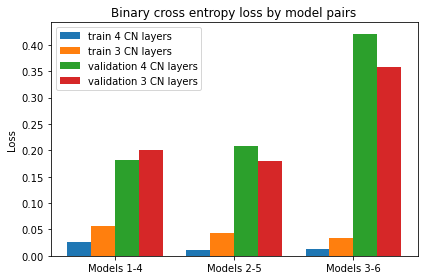
\includegraphics[width=0.4\textwidth]{images/loss.png}
    \caption{Loss per model during training and validation}
    \label{Lossgraph}
 \end{figure}
 \begin{figure}
    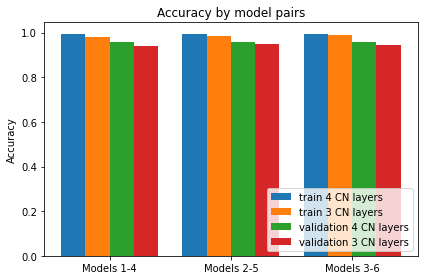
\includegraphics[width=0.4\textwidth]{images/ac.png}
    \caption{Accuracy per model during training and validation}
    \label{ACgraph}
\end{figure}

The performance during machine learning has been summarized in graph \ref{Lossgraph} and \ref{ACgraph}, and use the data found in \ref{ACtable}. These show a comparison of the models with 4 CN layers and the models with 3 CN layers in decreasing order of amount of dense layers.

\section{Discussion}
\subsection{GPU Resource Limitations and Impact on Results}
The limited availability of GPU resources has played a significant role in shaping the outcomes of this study, extending the training duration and inhibiting the development of highly sophisticated models. Furthermore, it has limited the number of data points obtained during training to accurately perform this overview. To thoroughly examine the relationship between model complexity and the emergence of double descent, future investigations should allocate substantial GPU resources, enabling in-depth analysis of various model configurations and their performance.

\subsection{Existing Knowledge Gaps and the Ambiguity of Double Descent}
The concept of double descent, first introduced in 2019 (\cite{Belkin2019ReconcilingTrade-off}), remains relatively novel, leading to several knowledge gaps in the field. As a result, some facets of the observed outcomes cannot be explained with absolute certainty, indicating that further research is needed to elucidate the intricacies of the double descent phenomenon. A hypothesis that has been adapted for the cause of double descent is the lottery ticket hypothesis. The hypothesis states that "A randomly initialized, dense neural network contains a sub-network that is initialized such that — when trained in isolation — it can match the test accuracy of the original network after training for at most the same number of iterations. \cite{Frankle2018TheNetworks}" The paper proposes that large enough neural networks that are randomly initialized, eventually find well-performing pathways called winning tickets during training. These tickets were isolated to test their existence via a technique called pruning which is basically removing parameters from the model as training continues. This lottery ticket hypothesis has been well documented and positive in findings for example in the Optimal brain damage (OBD) paper \cite{Denker2014OptimalDamage} and in \cite{Frankle2018TheNetworks}. Relating it back to double descent, A large enough model gives more chance of finding winning tickets. Therefore during training, the model first struggles to find winning tickets (the ascent) but once found, they increase the generalization and performance of the overall model (second descent). The winning tickets are only present during the second descent. Of course, to prove this hypothesis, further research has to be conducted perhaps only initializing pruning techniques when the second descent has been observed and documenting its performance on the loss curve.

\subsection{Impact of Hyperparameter Choices on Double Descent}
The choice of hyperparameters, such as learning rate, batch size, and regularization methods, can significantly influence the presence and prominence of the double descent curve. To gain a comprehensive understanding of the methodology, future studies should adopt a critical approach in evaluating optimal hyperparameter configurations for diverse model structures within the context of double descent, considering their potential effects on model performance.

\subsection{Assessing the Generalizability of Findings}
The present study primarily focuses on histopathology image analysis related to metastatic breast cancer, raising questions about the generalizability of the findings to other medical image analyses or different domains altogether. To ascertain the prevalence and applicability of the double descent phenomenon across multiple applications, subsequent research endeavors should extend their scope to include a variety of image analysis tasks and datasets. Double descent is however a general phenomenon in machine learning thus the focus of doing another research to study generalization should focus more on performance or architecture of the model on different tasks such as segmentation or multi-classification.

\subsection{Explanation of the AUC scores and the loss findings}
Models 1 and 3 are outperformed by models 4, 2, 5 and 6 in that order. With 6 being the simplest model trained for this case, these results do not support the claim that a double descent or a more complex model automatically lead to a better performance on the test set. It was decided that because of technical limitations regarding GPU usage and training time, that the most complex model that could be created within reason was one with 4 convolutional layers and 3 dense layers. However, reduction of parameters meant that some dense layers needed to be removed but that only results into 3 data points to describe the relation complexity has on the double descent phenomenon. To compensate for that, even more simplification was induced by removing a convolutional layer. However, removing a CN layer removes more weights than a dense layer and has other effects due to the reduction of filters. The only way to compare the models was to compare the one with an extra CN layer (model 1, 2 and 3 as the ones capable of double descent) to the ones who were over simplified to show any sign of that phenomenon (model 4, 5 and 6). One thing in common is that all models with 4 CN layers, have been outperformed by their counterpart which could mean that for this classification task and dataset combination, A lower amount of filters, is actually better suited because increasing the filters used might abstract the data in such a way that it results in increased validation loss and decreased test performance. Still, model 2 represented the best case of double descent and it also obtained the highest AUC score of the 3 that with 4 CN layers. Why model 2 shows a better double descent than model 1 is still unclear but it might be the fact that with every dense layer dropped, a dropout layer was also removed in our experiment. Dropout layers are mechanisms to reduce overfitting of the data. We inserted the dropout layer to introduce more variance in the model and to slightly boost the training time of the model as well. However, using dropout layers does reduce the chance of overfitting which might impact the ability for a loss curve to display a double descent. More dropout layers like in model 1 would therefore hurt the double descent instead of adding complexity. This should be tested by running the models with and without dropout layers and documenting the effect on double descent in further research.

\subsection{Influence of Data Preprocessing and Augmentation on Double Descent}
The impact of data preprocessing and augmentation techniques on the double descent curve constitutes a critical area of inquiry. Preprocessing procedures, such as normalization, resizing, and data augmentation, could potentially affect the model's performance and vulnerability to double descent. An in-depth investigation of the interplay between data preprocessing and model complexity is essential to derive best practices for mitigating the effects of double descent in real-world applications.

\subsection{Exploration of Alternative Deep Learning Architectures}
Finally, to understand the double descent phenomenon comprehensively, it is crucial to examine alternative deep learning architectures, including DenseNets, Inception networks, or Transformer-based models. This analysis will help determine if the double descent phenomenon is more optimal to convolutional neural networks (CNNs) or if it presents a higher occurrence and or performance in other deep learning models. By critically examining various architectures, researchers can gain insights into the underlying mechanisms responsible for the double descent phenomenon and identify optimal design choices for a wide range of model architectures, ultimately contributing to the development of more robust and effective solutions across diverse applications.

\section{Conclusion}
\subsection{Empirical Validation}
This study presents persuasive empirical evidence supporting the presence of the double descent phenomenon in convolutional neural networks (CNNs) employed for the demanding task of detecting metastasis in breast cancer patients. The outcomes from the loss curves \ref{model 1} \ref{model 2} corroborate previous findings on double descent, underscoring the significance of adequate depth, over-parameterization, and comprehensive datasets in unveiling this captivating behavior.

\subsection{Impact of Complexity on Double Descent}
A link was identified between the clarity of the double descent curve and the complexity of the neural network, implying that as the model's intricacy escalates, the double descent phenomenon becomes more pronounced. This finding bolsters the notion that leveraging deeper and extensively over-parameterized models can improve performance \ref{model 2}, contrary to the prevalent belief that increasing complexity would result in diminishing returns.

\subsection{Determining Stopping Points}
Moreover, the results indicate that for less complex models, establishing stopping conditions within the traditional regime is sufficient, as these models frequently lack the ability to replicate the epoch-wise double descent curve. These early-stopping conditions maintain generalization in the model allowing for broader application in other datasets.

\subsection{Enhanced Comprehension}
This investigation contributes to a more profound understanding of the delicate interconnection between model complexity, generalization, and performance within the realm of medical image analysis. Gaining such insights is vital for optimizing neural network architectures in real-world applications, especially when addressing high-stakes tasks like detecting metastases in cancer patients. This research lays the foundation for future in-depth analysis and fine-tuning of the methodology, fostering a more robust comprehension of the double descent phenomenon and its implications across a variety of applications.



% if have a single appendix:
%\appendix[Proof of the Zonklar Equations]
% or
%\appendix  % for no appendix heading
% do not use \section anymore after \appendix, only \section*
% is possibly needed

% use appendices with more than one appendix
% then use \section to start each appendix
% you must declare a \section before using any
% \subsection or using \label (\appendices by itself
% starts a section numbered zero.)
%


\appendices
\section{accuracy and loss tables}
Models 1, 2 and 3 contain 4 convolutional layers where 2 and 3 are missing 1 and 2 dense and dropout layers respectively.
Models 4, 5 and 6 contain 3 convolutional layers where 5 and 6 are missing 1 and 2 dense and dropout layers respectively
\begin{table}[h]
\centering
\begin{tabular}[width=0.7\textwidth]{|c|c|c|c|c|}
\hline
\textbf{Model} & \textbf{Train AC} & \textbf{Val AC} & \textbf{Train Loss} & \textbf{Val Loss} \\ \hline
1 & 0.9917 & 0.9574 & 0.02562 & 0.182 \\ \hline
2 & 0.994 & 0.9573 & 0.0117 & 0.2091 \\ \hline
3 & 0.9958 & 0.9556 & 0.01292 & 0.4217 \\ \hline
4 & 0.9809 & 0.9406 & 0.05571 & 0.2011 \\ \hline
5 & 0.9836 & 0.9475 & 0.04287 & 0.1801 \\ \hline
6 & 0.987 & 0.9429 & 0.03409 & 0.3589 \\ \hline
\end{tabular}
\label{ACtable}
\caption{Summary of Training and Validation Metrics for CNN example in assignment 3}
\end{table}
\newpage
% you can choose not to have a title for an appendix
% if you want by leaving the argument blank
\section{Code}


\section{Accuracy and Loss Curves}
See next page.
\begin{figure*}[!t]
\centering
\subfloat[1]{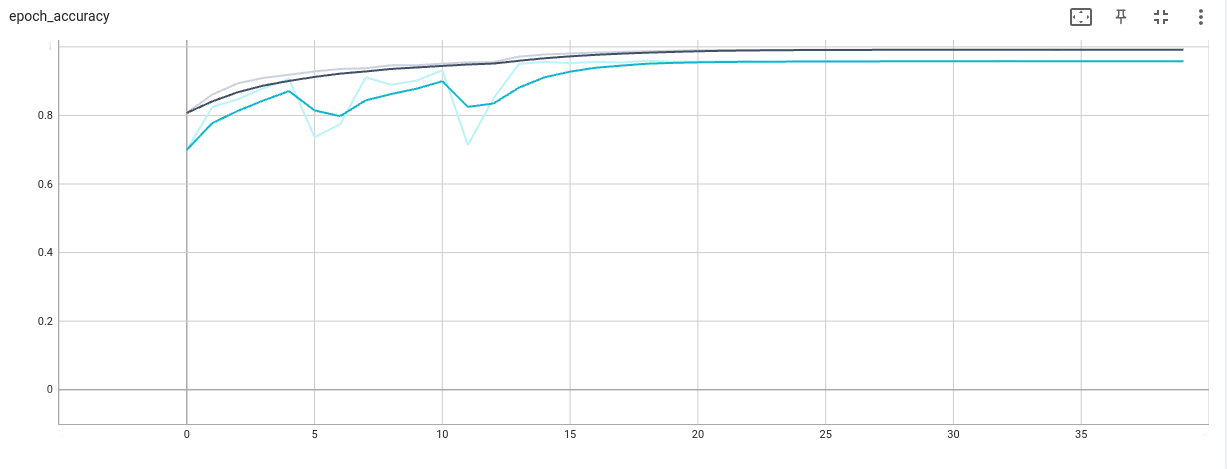
\includegraphics[angle=90, height=25cm, width=0.4\textwidth]{images/1_ac.png}}
\hfil
\subfloat[2]{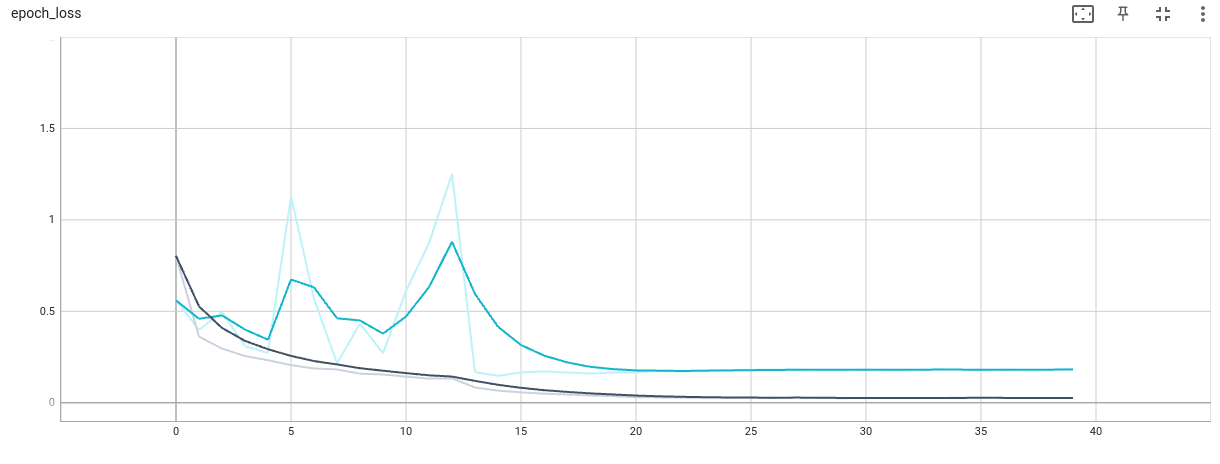
\includegraphics[angle=90, height=25cm, width=0.4\textwidth]{images/1_loss.png}
\caption{Model 1.}}
\label{model 1}
\end{figure*}

\begin{figure*}[!t]
\centering
\subfloat[1]{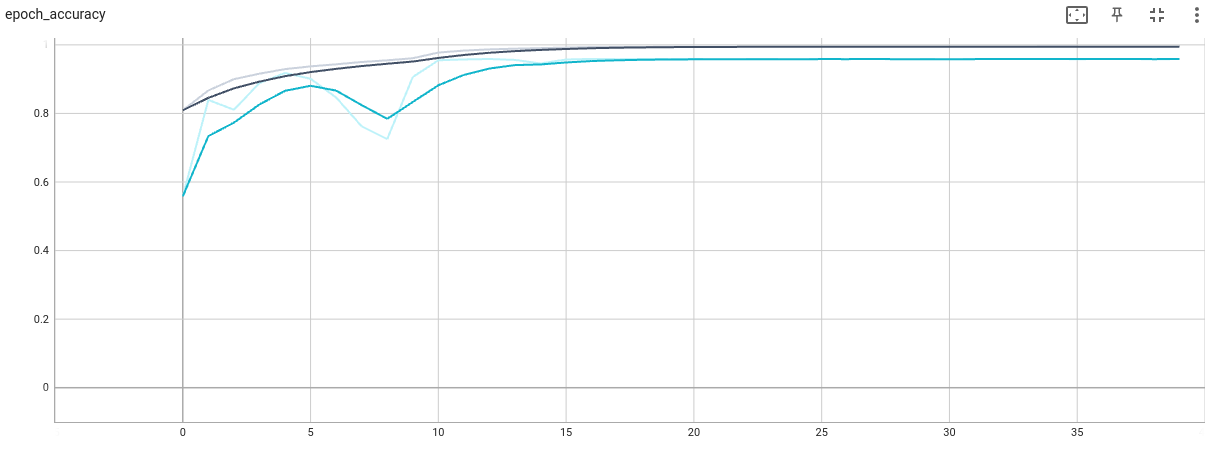
\includegraphics[angle=90, width=0.4\textwidth]{images/2_ac.png}}
\hfil
\subfloat[2]{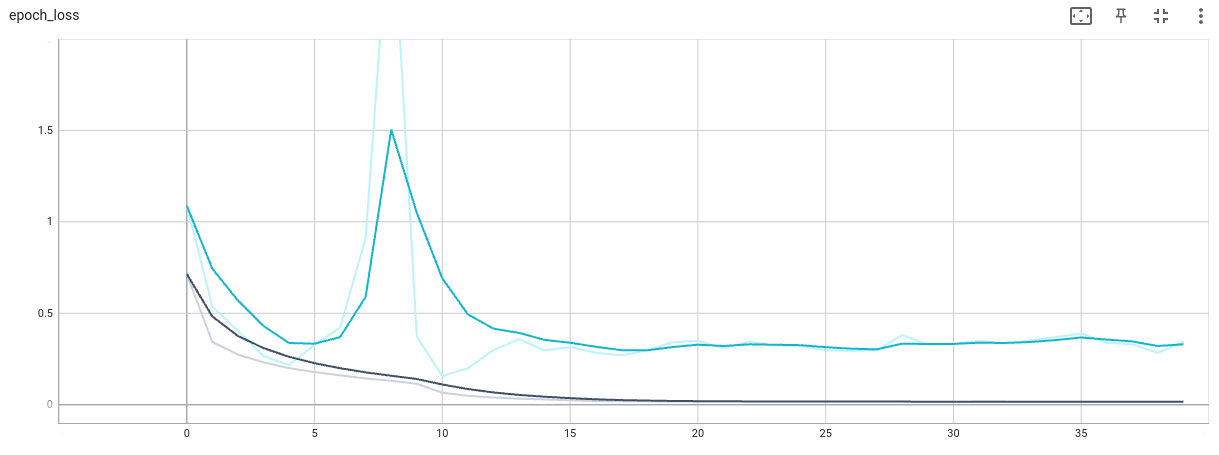
\includegraphics[angle=90, width=0.4\textwidth]{images/2_loss.png}
\caption{Model 2.}}
\label{model 2}
\end{figure*}

\begin{figure*}[!t]
\centering
\subfloat[1]{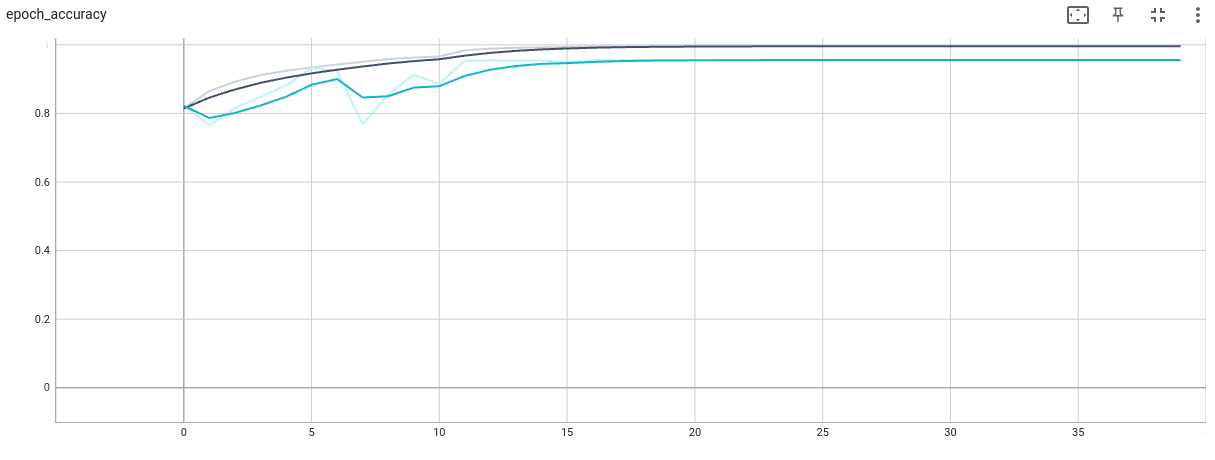
\includegraphics[angle=90, width=0.4\textwidth]{images/3_ac.png}}
\hfil
\subfloat[2]{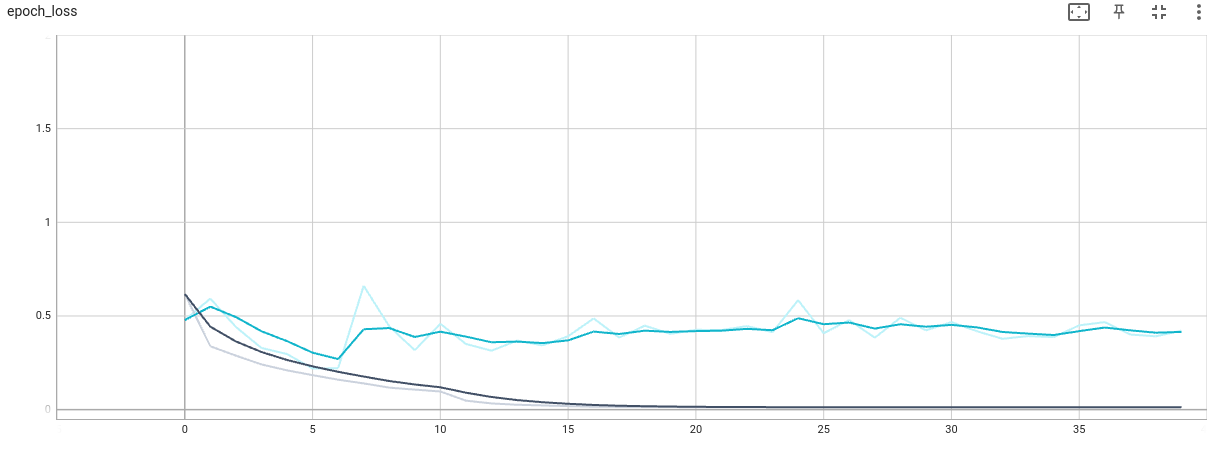
\includegraphics[angle=90, width=0.4\textwidth]{images/3_loss.png}
\caption{Model 3.}}
\label{model 3}
\end{figure*}

\begin{figure*}[!t]
\centering
\subfloat[1]{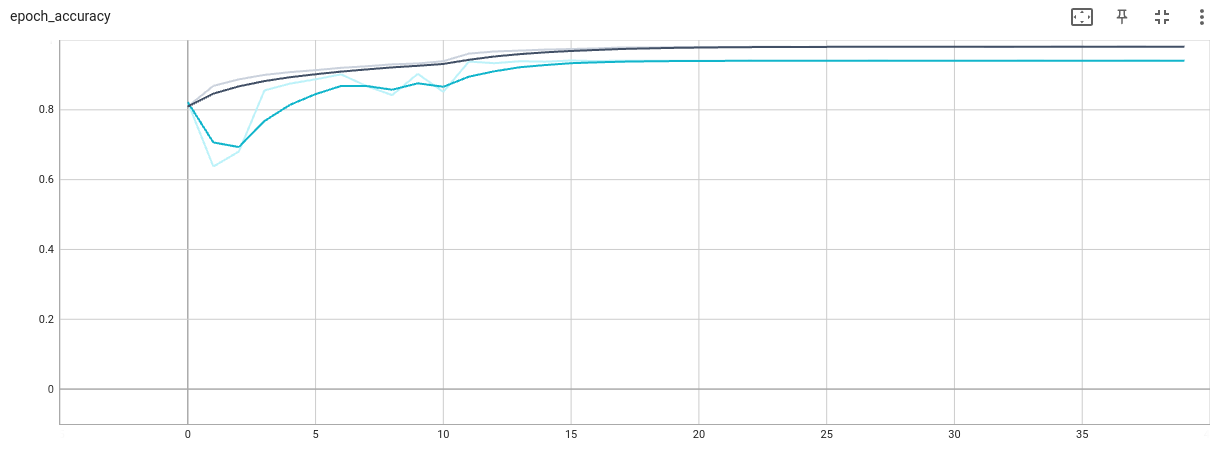
\includegraphics[angle=90, width=0.4\textwidth]{images/4_ac.png}}
\hfil
\subfloat[2]{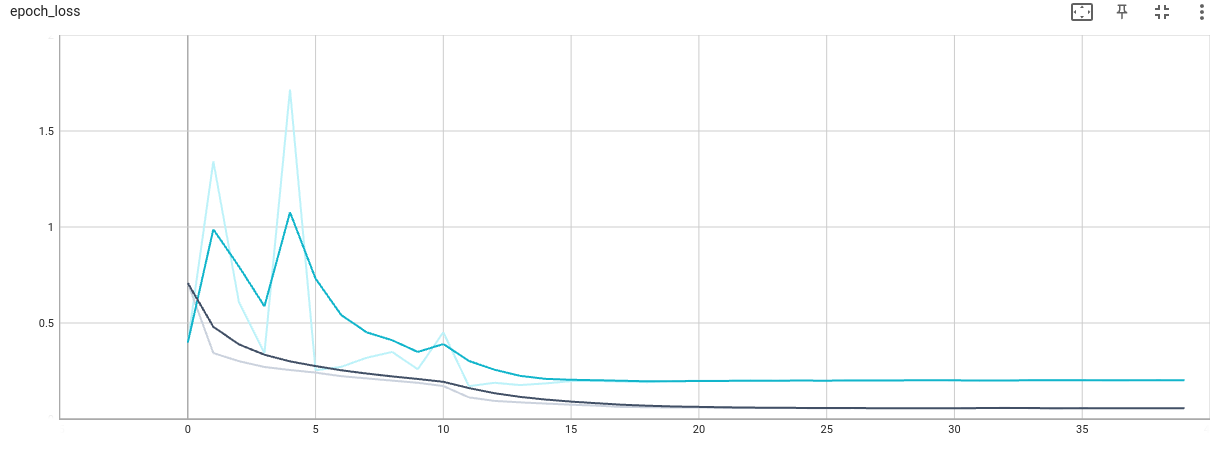
\includegraphics[angle=90, width=0.4\textwidth]{images/4_loss.png}
\caption{Model 4.}}
\label{model 4}
\end{figure*}

\begin{figure*}[!t]
\centering
\subfloat[1]{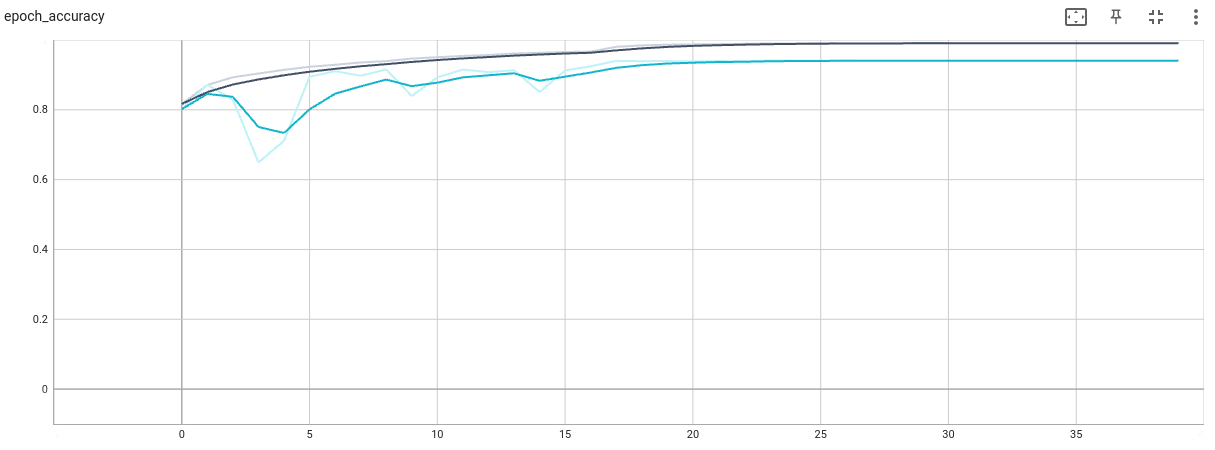
\includegraphics[angle=90, width=0.4\textwidth]{images/5_ac.png}}
\hfil
\subfloat[2]{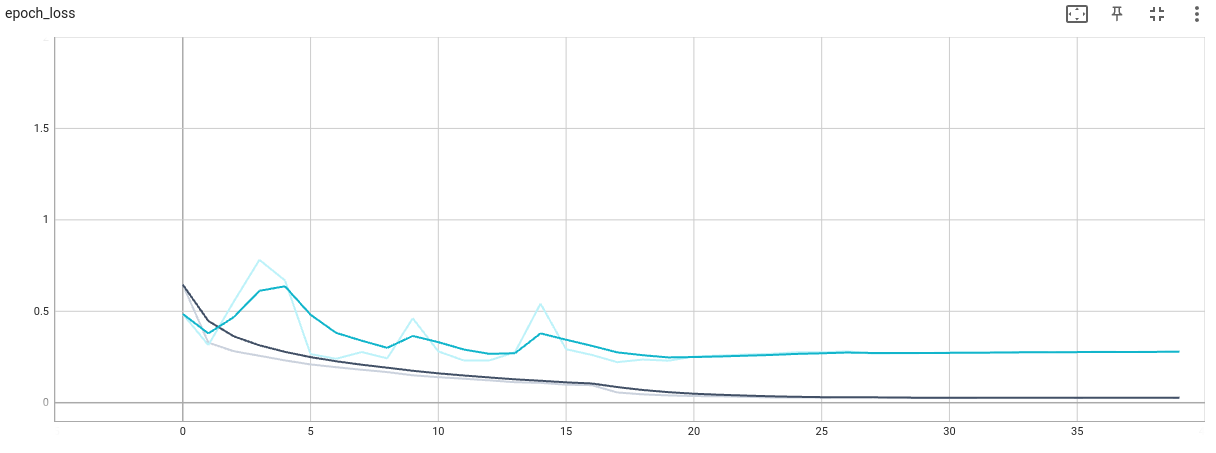
\includegraphics[angle=90, width=0.4\textwidth]{images/5_loss.png}
\caption{Model 5.}}
\label{model 5}
\end{figure*}

\begin{figure*}[!t]
\centering
\subfloat[1]{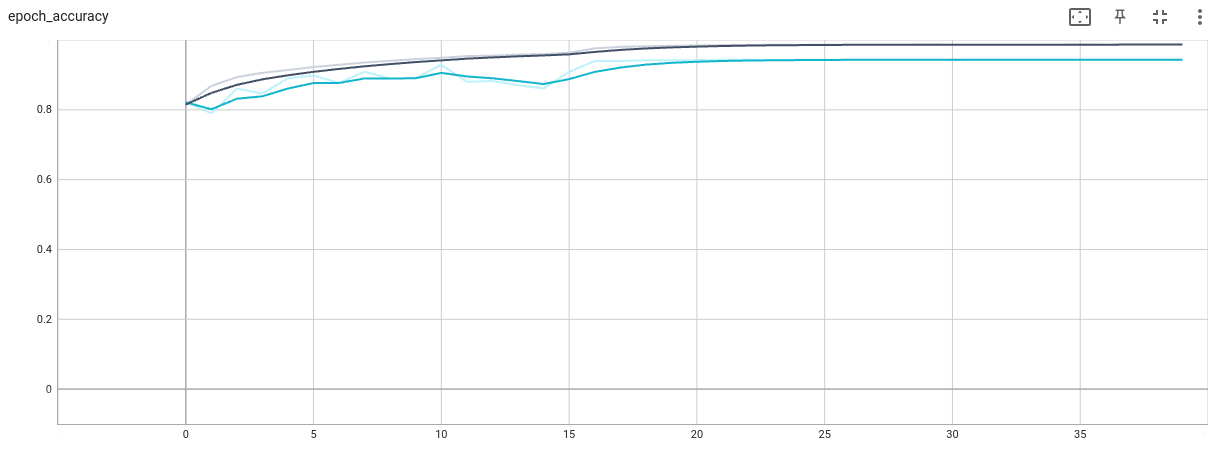
\includegraphics[angle=90, width=0.4\textwidth]{images/6_ac.png}}
\hfil
\subfloat[2]{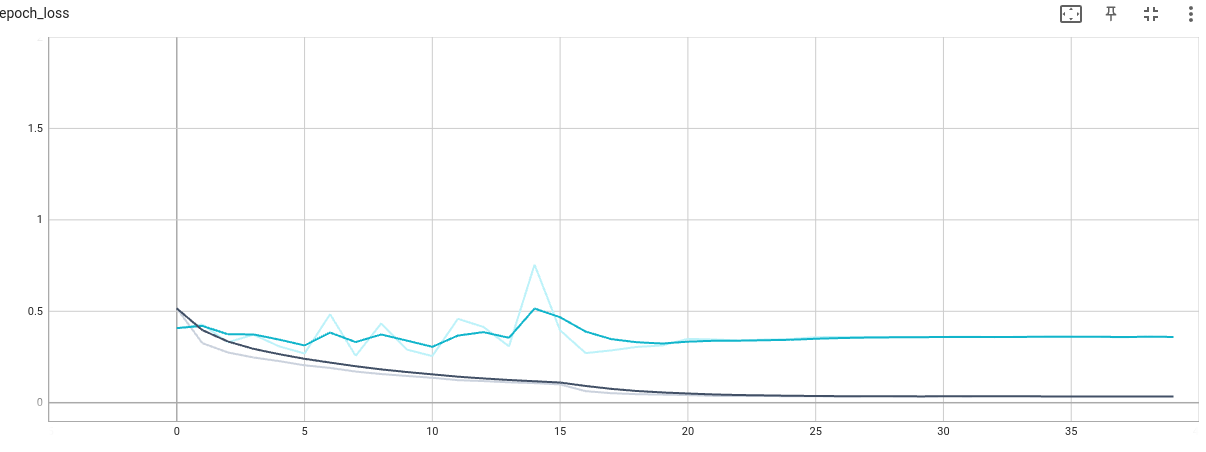
\includegraphics[angle=90, width=0.4\textwidth]{images/6_loss.png}
\caption{Model 6.}}
\label{model 6}
\end{figure*}


% use section* for acknowledgment
\ifCLASSOPTIONcompsoc
  % The Computer Society usually uses the plural form
  \section*{Acknowledgments}
\else
  % regular IEEE prefers the singular form
  \section*{Acknowledgment}
\fi


The authors would like to thank assistant professor at the medical image analysis group Mitko Veta for being our project manager and Stefan Rademakers as our TA for their continuous support in this endeavour.


% Can use something like this to put references on a page
% by themselves when using endfloat and the captionsoff option.
\ifCLASSOPTIONcaptionsoff
  \newpage
\fi



% trigger a \newpage just before the given reference
% number - used to balance the columns on the last page
% adjust value as needed - may need to be readjusted if
% the document is modified later
%\IEEEtriggeratref{8}
% The "triggered" command can be changed if desired:
%\IEEEtriggercmd{\enlargethispage{-5in}}

% references section

% can use a bibliography generated by BibTeX as a .bbl file
% BibTeX documentation can be easily obtained at:
% http://mirror.ctan.org/biblio/bibtex/contrib/doc/
% The IEEEtran BibTeX style support page is at:
% http://www.michaelshell.org/tex/ieeetran/bibtex/
%\bibliographystyle{IEEEtran}
% argument is your BibTeX string definitions and bibliography database(s)
%\bibliography{IEEEabrv,../bib/paper}
%
% <OR> manually copy in the resultant .bbl file
% set second argument of \begin to the number of references
% (used to reserve space for the reference number labels box)


% Bibliography
\begin{References}

%\bibitem{IEEEhowto:kopka}
%H.~Kopka and P.~W. Daly, \emph{A Guide to {\LaTeX}}, 3rd~ed.\hskip 1em plus
%  0.5em minus 0.4em\relax Harlow, England: Addison-Wesley, 1999.

\printbibliography
\end{References}



% biography section
% 
% If you have an EPS/PDF photo (graphicx package needed) extra braces are
% needed around the contents of the optional argument to biography to prevent
% the LaTeX parser from getting confused when it sees the complicated
% \includegraphics command within an optional argument. (You could create
% your own custom macro containing the \includegraphics command to make things
% simpler here.)
%\begin{IEEEbiography}[{\includegraphics[width=1in,height=1.25in,clip,keepaspectratio]{mshell}}]{Michael Shell}
% or if you just want to reserve a space for a photo:



% insert where needed to balance the two columns on the last page with
% biographies
%\newpage


% You can push biographies down or up by placing
% a \vfill before or after them. The appropriate
% use of \vfill depends on what kind of text is
% on the last page and whether or not the columns
% are being equalized.

%\vfill

% Can be used to pull up biographies so that the bottom of the last one
% is flush with the other column.
%\enlargethispage{-5in}



% that's all folks
\end{document}


